\documentclass[11pt]{article}

\usepackage[review]{acl}

\usepackage{times}
\usepackage{latexsym}
\usepackage[T1]{fontenc}
\usepackage[utf8]{inputenc}
\usepackage{microtype}
\usepackage{inconsolata}
\usepackage{graphicx}
\usepackage{booktabs}
\usepackage{multirow}
\usepackage{enumitem}
\usepackage{amsmath}
\usepackage{xcolor}
\usepackage{pgfplots}
\pgfplotsset{compat=1.18}
\usepgfplotslibrary{groupplots}
\usetikzlibrary{arrows.meta, positioning}

% Espacement resserre autour des flottants et des legendes, pour tenir le corps en huit pages.
\setlength{\textfloatsep}{8pt plus 2pt minus 2pt}
\setlength{\floatsep}{6pt plus 2pt minus 2pt}
\setlength{\dbltextfloatsep}{8pt plus 2pt minus 2pt}
\setlength{\dblfloatsep}{6pt plus 2pt minus 2pt}
\setlength{\intextsep}{6pt plus 2pt minus 2pt}
\setlength{\abovecaptionskip}{4pt}
\setlength{\belowcaptionskip}{-2pt}

% \autoref doit nommer les sections avec une majuscule, comme Table et Figure.
\renewcommand{\sectionautorefname}{Section}
\renewcommand{\subsectionautorefname}{Section}
% \autoref pour deux cibles : le lien couvre le nom au pluriel et le premier numero, comme \autoref.
\newcommand{\autorefpair}[3]{\hyperref[#2]{#1~\ref*{#2}} and~\hyperref[#3]{\ref*{#3}}}

\title{Unrelated Is Not Opposed:\\A Signed Scale for Meaning Preservation}

\author{Anonymous Submission}
\date{}

\begin{document}
\maketitle

\begin{abstract}
Meaning preservation metrics output a non-negative score and therefore cannot represent opposition. For example, MeaningBERT scores ``I drink milk'' and ``I do not drink milk'' at $58.30$ out of $100$, although the two sentences state opposite facts.
We propose a signed scale on $[-100, 100]$ that combines two scores: that of an existing similarity metric, which measures how close in meaning two sentences are, and that of a polarity head, a classifier that estimates the probability that one sentence contradicts the other. The similarity score is weighted down as this probability rises and becomes negative when a contradiction is likely, so that unrelated sentences score 0 and contradictions receive a negative score.
We train the polarity head on inference data, and adding generated identical, unrelated and opposite pairs to its training data makes it reliable at both ends of the scale.
Combined with an existing metric, which needs no retraining, the signed score places most contradictions below zero and accepts nearly seven times fewer contradictions as meaning-preserving at a fixed threshold.
\end{abstract}

\section{Introduction}
\label{sec:intro}

Assessing whether a rewritten sentence preserves the meaning of its source is a prerequisite for evaluating text simplification, summarization, and translation \citep{saggion2017automatic}.
The metrics designed for this purpose, whether embedding-based (e.g. Sentence-BERT \citep{reimers2019sbert} or BERTScore \citep{zhang2020bertscore}), question-based (e.g. QuestEval \citep{scialom2021questeval}) or trained end to end (e.g. LENS \citep{maddela2023lens} or MeaningBERT \citep{beauchemin2023meaningbert}), all return a single non-negative number, typically ranging from $100$ for sentences with identical meanings to $0$ for those with completely different meanings.

This output cannot represent opposition.
Two sentences that contradict each other are about the same topic, so they share most of their words and concepts, and a metric that measures how much meaning two sentences share reads that overlap as preserved meaning.
For example, MeaningBERT scores the sentences ``I drink milk'' and ``I do not drink milk'' at $58.30$ out of $100$, in the higher half of the scale, indicating that meaning is preserved between the two.
\citet{baral2026lexflip} observed the same effect on legal text: perturbations that reverse the legal force of a sentence while preserving most of its tokens have only a minor impact on embedding metrics.

Separating agreement from contradiction requires a quantity that a non-negative score does not carry: whether the two sentences discussing the same topic assert the same facts or their opposites.
We therefore propose a signed scale on $[-100, 100]$, on which $100$ denotes two sentences with identical meanings, $0$ two unrelated sentences, and negative values two related sentences that assert opposite facts. We obtain this score by composing the score of a similarity metric with a separately-trained polarity head.
Our contributions are:

\begin{enumerate}[nosep]
\item A meaning preservation metric on a signed scale that distinguishes opposed meaning from unrelated meaning (\autorefpair{Sections}{sec:scale}{sec:composition}).
\item A polarity head and the stratified, leakage-free corpus with derived-polarity data augmentation on which it is trained (\autorefpair{Sections}{sec:data}{sec:results}).
\end{enumerate}

\section{Related Work}
\label{sec:related}

\subsection{Meaning Preservation Metrics}

Meaning preservation metrics can be divided into three families.
First, embedding-based metrics compare sentence representations. For example, Sentence-BERT computes the cosine between two sentence embeddings, and BERTScore matches each token of a sentence to its most similar counterpart in the other sentence.
A negation can add as little as a single token to an otherwise identical sentence, which barely changes either score.
Second, question-based metrics such as QuestEval generate questions from one text and check whether the other answers them. A negated sentence, which mentions the same entities as the original text, can answer most generated questions.
Third, learned metrics such as LENS and MeaningBERT are trained to replicate human ratings, for overall simplification quality in the former case and for meaning preservation in the latter.
These ratings range from identical meaning down to no shared meaning, with no value for opposite meaning: an annotator can only rate a contradicting pair low, at the end of the scale reserved for unrelated pairs. The training signal therefore offers no way to separate the two, and in practice the learned metric does not even score contradictions low: MeaningBERT scores ``I drink milk'' and ``I do not drink milk'' at $58.30$ (\autoref{sec:intro}).

All these metrics output a non-negative magnitude and are validated by correlation with human ratings. MeaningBERT further introduced two sanity checks, under which identical sentences must score $100$ and unrelated sentences $0$. 
None test opposition: any monotone function of lexical overlap satisfies both checks \citep{baral2026lexflip}, and a correlation with ratings that do not distinguish a contradiction from a poor paraphrase cannot reward a metric that does.
Specialized metrics, for legal text \citep{beauchemin2025judgebert} and biomedical simplification \citep{lyu2024scigispy}, show that general metrics miss small edits with large consequences, but they too output a non-negative score.
Rather than replace these metrics, we use one as the similarity component of a signed score and supply the missing direction separately (\autoref{sec:scale}).

\subsection{Natural Language Inference}

Natural language inference provides the polarity that preservation metrics lack.
Large-scale corpora \citep{williams2018mnli,nie2020anli} and fact-verification datasets \citep{thorne2018fever,schuster2021vitaminc} label sentence pairs as entailment, neutral or contradiction, and targeted suites such as MoNLI \citep{geiger2020monli} and NaN-NLI \citep{truong2022nannli} probe negation.
The two tasks answer complementary questions: an inference model states whether the second sentence follows from or denies the first but not how much meaning the two share, whereas a preservation metric measures the shared meaning but not its entailment relationship.
We therefore combine the two rather than replace one with the other (\autoref{sec:scale}).
To our knowledge, SICK \citep{marelli2014sick} is the only resource annotating both measures over the same pairs, which is why it serves to evaluate the combination.
Inference models already serve evaluation: SummaC \citep{laban2022summac} and AlignScore \citep{zha2023alignscore} detect inconsistency between a summary and its source, and MENLI \citep{chen2023menli} combines inference scores with similarity metrics to resist adversarial edits such as negation.
These metrics still output a non-negative score; ours keeps the similarity metric and makes the score signed, so that an unrelated pair stays at $0$ and a contradiction falls below it.

\section{A Signed Scale}
\label{sec:scale}

Meaning metrics use an unsigned scale on which $100$ denotes identical meaning and $0$ denotes unrelated sentences, the two anchors of the sanity checks of \citet{beauchemin2023meaningbert}. We propose a signed scale on $[-100, 100]$. Its positive half is the unsigned scale with both anchors unchanged, so a non-negative score reads as it does on a meaning metric. Its negative half denotes opposite meaning: the sign carries polarity and the absolute value the closeness of the two sentences, so $-100$ denotes a pair as close as possible in content that asserts the opposite. 
%The decisive property is that the negative half measures active contradiction rather than the absence of shared meaning: two sentences about different topics score $0$, not $-100$, since to contradict each other they must first be about the same thing.
Our score therefore carries two quantities: the magnitude measures how close the two sentences are in content, and the polarity whether they assert the same thing.
We compose the two as
\begin{equation}
s = m \times (1 - 2\, p_{\mathrm{contra}}),
\label{eq:compose}
\end{equation}
with $m \in [0,100]$ the score of any similarity metric and $p_{\mathrm{contra}} \in [0,1]$ the probability of contradiction given by a polarity head.
The polarity head is a classifier that reads the two sentences and, as in natural language inference, outputs a probability for each of three classes: entailment, neutral and contradiction.
Only $p_{\mathrm{contra}}$ enters \autoref{eq:compose}, and \autorefpair{Sections}{sec:data}{sec:setup} describe how we train the head.
The form is a product and not a difference: an unrelated pair has $m \approx 0$ and scores near zero whatever its polarity, whereas a subtraction would let it drift negative and destroy the distinction the scale rests on.
\autoref{tab:scale} illustrates the behavior the scale aims for on five sample cases.
%, and \autoref{fig:pipeline} traces one of them through both heads.

One may object that a negation is closer in meaning to its source than an unrelated sentence, so that $100$, $50$ and $0$ would be a defensible order for a paraphrase, a contradiction and an unrelated pair.
The signed scale keeps that closeness in $|s|$: on the $1$--$5$ relatedness scale of SICK, human raters place contradictions at $3.59$ on average against $2.98$ for neutral pairs, in line with the long-standing observation that opposites are semantically close \citep{mohammad2013contrast,hill2015simlex}.
What an unsigned order cannot carry is the direction, since a contradiction and a paraphrase that kept half of its content would both land near $50$.
Placing contradictions below zero also reflects their cost when a metric decides whether a rewrite may replace its source: an unrelated output is visible to the reader, whereas a negation misleads, and factual errors are a central risk of rewriting \citep{maynez2020faithfulness}, to the point that an inaccurate simplification may be worse than none \citep{devaraj2022factuality}.

\begin{table}[t]
\centering\small
\begin{tabular}{p{2.85cm} ccc}
\toprule
Pair & $m$ & $p_{\mathrm{contra}}$ & $s$ \\
\midrule
``I drink milk'' / ``I consume milk'' & 95.00 & 0.01 & $+93.10$ \\
\addlinespace
``I drink milk'' / ``My sister drinks milk'' & 50.00 & 0.05 & $+45.00$ \\
\addlinespace
``I drink milk'' / ``I rarely drink milk'' & 70.00 & 0.50 & $0.00$ \\
\addlinespace
``I drink milk'' / ``the meeting is at three'' & 0.00 & 0.05 & $0.00$ \\
\addlinespace
``I drink milk'' / ``I do not drink milk'' & 60.00 & 0.99 & $-58.80$ \\
\bottomrule
\end{tabular}
\caption{Intended behavior of the scale on illustrative examples: $m$ stands for any similarity metric and $p_{\mathrm{contra}}$ for a learned polarity head.}
\label{tab:scale}
\end{table}

%% Figure ecrite a la main : les chiffres viennent des memes mesures que le tableau 1.
\begin{figure}[t]
\centering
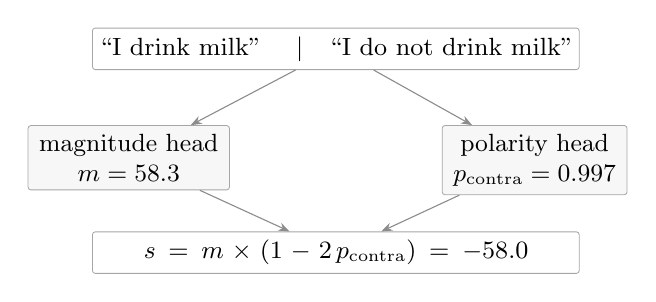
\begin{tikzpicture}[
  font=\small,
  box/.style={draw=black!35, line width=0.3pt, rounded corners=1pt,
              inner xsep=4pt, inner ysep=3pt, align=center},
  head/.style={box, fill=black!3},
  flow/.style={-{Stealth[length=4pt]}, draw=black!45, line width=0.4pt},
]
\node[box, text width=5.9cm] (pair)
  {``I drink milk'' \quad\textbar\quad ``I do not drink milk''};

\node[head, below left=0.7cm and -1.75cm of pair] (mag)
  {magnitude head\\$m = 58.3$};
\node[head, below right=0.7cm and -1.75cm of pair] (pol)
  {polarity head\\$p_{\mathrm{contra}} = 0.997$};

\node[box, below=2.05cm of pair, text width=5.9cm] (out)
  {$s = m \times (1 - 2\,p_{\mathrm{contra}}) = -58.0$};

\draw[flow] (pair) -- (mag);
\draw[flow] (pair) -- (pol);
\draw[flow] (mag) -- (out);
\draw[flow] (pol) -- (out);

\end{tikzpicture}
\caption{One pair, end to end. The two heads are read independently and the composition of \autoref{eq:compose} turns a middling positive score into a negative one. The same pipeline on ``I drink milk'' against ``I consume milk'' gives $m = 96.7$, $p_{\mathrm{contra}} = 0.005$ and $s = +95.8$, and on an unrelated pair $m = 0.0$ sends the product to zero whatever the polarity says.}
\label{fig:pipeline}
\end{figure}


The factor $2$ is what makes the scale symmetric, and it follows from the definition rather than from a fit.
Writing $1 - 2\,p_{\mathrm{contra}} = (1 - p_{\mathrm{contra}}) - p_{\mathrm{contra}}$ shows that $m$ is weighted by the margin between the probability that the pair does not contradict and the probability that it does.
A certain non-contradiction leaves $m$ unchanged and a certain contradiction maps it to $-m$, so the closeness of the pair is kept on either side of zero and only the sign changes, and $s$ stays within $[-m, m]$, hence within $[-100, 100]$ with no clipping.
The sign flips at $p_{\mathrm{contra}} = 0.5$, where the head finds contradiction as likely as not: the pair at $0.50$ in \autoref{tab:scale} is related, but the head cannot tell its direction, so the scale withholds a verdict and scores it $0$.
A smaller factor would truncate the negative half, since a certain contradiction would then land at $-m/2$ with a factor of $1.5$, and a larger one would flip the sign on weaker evidence and saturate at $-100$; \autoref{sec:composition} measures both.
The negation stays at $-58.80$ rather than near $-100$ because the similarity metric already lowered $m$ for the negation it partly detects, so $|s|$ understates how close the pair is.

\section{Data}
\label{sec:data}

\subsection{What Each Corpus Contributes}

Building the signed score requires three things from the data: a high volume of inference pairs to train the polarity head, a corpus annotated with both relatedness and inference over the same pairs to study how $m$ and $p_{\mathrm{contra}}$ combine, and targeted sets that expose the failures an aggregate score hides.
No single corpus provides all three, so we draw from five corpora; \autoref{tab:corpora} presents their size, labels and use.

VitaminC \citep{schuster2021vitaminc} supplies the volume, and in the regime this paper targets.
Its 488{,}904 pairs are contrastive by construction: a Wikipedia sentence was edited so that the claim its previous revision supported is refuted by the next, which produces contradictions differing from their source by a few tokens rather than by topic.
SICK \citep{marelli2014sick} links the two quantities, since it carries a relatedness score and an inference label over the same pairs.
MoNLI \citep{geiger2020monli} and NaN-NLI \citep{truong2022nannli} probe negation.
MoNLI contains 1{,}202 pairs that differ by a single word replaced with a more general or more specific one, under a negation that reverses the direction of entailment: ``There is a man not wearing a hat'' entails ``There is a man not wearing a sunhat'', whereas without the negation the entailment runs the other way.
NaN-NLI contains 258 pairs written to target negation below the clause level, where it scopes over a quantifier or a phrase rather than over the whole sentence, as in ``Not all people have had the opportunities you have had'' and ``Some people have not had the opportunities you have had''.
They never enter training and serve as held-out sets for negation (\autoref{tab:final}), because a head that scores well on VitaminC while failing them has learned the corpus and not the relation.
Last, CSMD \citep{beauchemin2023meaningbert}, the corpus of continuous-scaled human meaning preservation ratings on which MeaningBERT was trained, supplies 407 test pairs that serve to check the signed scale on simplification output.

\begin{table}[t]
\centering\small
\begin{tabular}{l r l l}
\toprule
Corpus & Rows & Labels & Use \\
\midrule
VitaminC & 488{,}904 & \textsc{fact3} & train/dev/test \\
SICK & 9{,}840 & \textsc{nli3} + rel. & train/dev/test \\
MoNLI & 1{,}202 & ent./neutral & held-out \\
NaN-NLI & 258 & \textsc{nli3} & held-out \\
CSMD & 1{,}355 & rating 0--100 & scale check \\
\bottomrule
\end{tabular}
\caption{Corpora used, with their size, label scheme and role.}
\label{tab:corpora}
\end{table}

\subsection{Data Augmentation at the Ends of the Scale}

Inference corpora contain few identical pairs and unrelated pairs, since neither poses an interesting inference problem.
Yet these are the pairs on which a signed score must be exact: $100$ for a sentence paired with itself and $0$ for two sentences with nothing in common.
We therefore train under two conditions: \textsc{raw}, the merged corpus alone, and \textsc{aug}, the same corpus plus 25{,}000 generated pairs of each of three kinds.
An identical pair, $(A, A)$, is labeled entailment, so that a sentence paired with itself scores $100$.
An unrelated pair joins two training sentences drawn at random that share few tokens and is labeled neutral, so that unrelated sentences score $0$ rather than a negative value.
A mirrored contradiction swaps the order of an existing contradiction, $(B, A)$ for $(A, B)$, and keeps its label, so that a contradiction is detected in either order.

A generated pair receives a label only when that label follows from the original pair.
A contradiction survives the swap, since if $A$ contradicts $B$ then $B$ contradicts $A$.
An entailment does not: ``a dog is running'' entails ``an animal is running'', but the reverse is false, so the swapped pair has no known label and we mirror contradictions only.
Mirroring every contradiction would double that class, from 50{,}267 to 100{,}534 pairs against 50{,}602 entailments, and push the head to overfit on contradictions.
We therefore mirror a random sample of 25{,}000 contradictions, the same quota as for identical and unrelated pairs, so that each class grows by 25{,}000 and the three stay balanced, at 75{,}602 entailments, 76{,}191 neutral pairs and 75{,}267 contradictions (\autoref{tab:final}).

\subsection{Stratified Splits}

The development and test splits are stratified by class and by corpus.
Each contains 4{,}000 pairs per class, drawn equally from each corpus; a corpus too small for its share is taken whole, and the remainder is drawn from the others.
Without this stratification, VitaminC, fifty times larger than SICK, would leave SICK at $8.16\%$ of the test split, and model selection would rest almost entirely on Wikipedia claim-evidence pairs; with it, SICK makes up $34.30\%$ of the test split.
Since VitaminC reuses the same evidence sentence across many claims, we then remove from the development and training splits every pair whose source sentence also appears in a later split.
\autoref{tab:final} presents the resulting counts per split and class, and \autoref{an:corpus} the construction.

\begin{table}[t]
\centering\small
\begin{tabular}{l rrrr}
\toprule
Split & Ent. & Neutral & Contra. & Total \\
\midrule
\multicolumn{5}{l}{\emph{Training, differs by condition}} \\
\textsc{raw} & 50{,}602 & 51{,}191 & 50{,}267 & 152{,}060 \\
\textsc{aug} & 75{,}602 & 76{,}191 & 75{,}267 & 227{,}060 \\
\multicolumn{5}{l}{\emph{Evaluation, identical for \textup{\textsc{raw}} and \textup{\textsc{aug}}}} \\
Dev & 3{,}939 & 3{,}864 & 3{,}968 & 11{,}771 \\
Test & 4{,}000 & 4{,}000 & 4{,}000 & 12{,}000 \\
Sanity & 1{,}500 & 1{,}500 & 1{,}500 & 4{,}500 \\
\multicolumn{5}{l}{\emph{Held-out, never trained on}} \\
MoNLI & 601 & 601 & -- & 1{,}202 \\
NaN-NLI & 97 & 44 & 117 & 258 \\
\bottomrule
\end{tabular}
\caption{Final polarity data per split and class. \textsc{aug} adds 25{,}000 identical pairs, unrelated pairs and mirrored contradictions to \textsc{raw}. We use the same splits for the dev, test and sanity suites.}
\label{tab:final}
\end{table}

\section{Experimental Setup}
\label{sec:setup}

\paragraph{Encoders.}
We fine-tune the polarity head on seven pretrained encoders (\autoref{tab:main}), all encoder-only models that read the two sentences jointly, the standard architecture for sentence-pair classification.
They are chosen along two axes.
The first is the pretraining generation, from BERT \citep{devlin2019bert} to RoBERTa \citep{liu2019roberta} and DeBERTaV3 \citep{he2023debertav3}: \texttt{BERT-base} is the encoder of MeaningBERT and thus the natural starting point for a head meant to sit beside it, and DeBERTaV3 outperforms the other two on inference benchmarks at equal size \citep{he2023debertav3}.
The second is the task a checkpoint was already fine-tuned on: none, semantic similarity for \texttt{RoBERTa-base\textsubscript{STS-B}}, or inference for \texttt{RoBERTa-large\textsubscript{MNLI}} and the two \texttt{DeBERTa-v3\textsubscript{NLI}} checkpoints, which tests whether a model that already scores similarity or inference learns polarity more easily.
The inference checkpoints matter because the polarity head is itself a three-way inference classifier: a checkpoint already fine-tuned on inference corpora starts with a head trained on our three classes, and it is what a practitioner would reach for off the shelf (\autoref{an:zeroshot}).
Including them tests whether our corpus still adds anything over that starting point, and pairing each DeBERTaV3 size with its plain checkpoint isolates the effect of inference pretraining at constant size.
Checkpoints that already have a three-way inference head keep it, with its rows reordered when the published class order differs from ours.

\paragraph{Training.}
Each encoder is trained under both conditions of \autoref{sec:data}, \textsc{raw} with 152{,}060 training pairs and \textsc{aug} with 227{,}060, and each configuration is repeated over ten random seeds.
All runs share the same optimization settings, given with the hardware in \autoref{an:training}.

\paragraph{Evaluation.}
We report four measures.
Macro-F\textsubscript{1} \citep{sokolova2009systematic} on the test split of \autoref{tab:final} measures the three-way task.
The area under the ROC curve (AUC; \citealp{hanley1982auc}) of $1 - p_{\mathrm{contra}}$ at ranking entailment above contradiction, where $50\%$ is chance, measures the quantity the signed score consumes; for a similarity metric, the AUC ranks its score directly (\autoref{an:failure}).
Accuracy on three sanity suites, made of identical, unrelated and mirrored pairs generated as in \autoref{sec:data} from test-split sentences, checks the extreme ends of the scale.
Accuracy on the two held-out sets of \autoref{tab:final}, MoNLI and NaN-NLI, probes negation.

\paragraph{Baselines.}
Three baselines without a pretrained encoder bound the polarity head from below: \texttt{Majority}, \texttt{Jaccard} and \texttt{TF-IDF}.
\texttt{Majority} always predicts the same class.
\texttt{Jaccard} computes the Jaccard overlap \citep{jaccard1912} of the two sentences' word sets and predicts neutral below a first threshold, contradiction between the two thresholds and entailment above the second, both fitted on the development split.
\texttt{TF-IDF} trains a logistic regression on the word unigrams and bigrams of the two sentences.

\paragraph{Statistics.}
We compare \textsc{raw} and \textsc{aug} for each encoder with Welch's $t$-test \citep{welch1947} over the ten random seeds, and two encoders with a paired $t$-test matched by random seed.
Every $p$-value comes with Cohen's $d$, because with ten random seeds and standard deviations near $0.20$ points, a difference of $0.10$ points can be significant yet negligible.
Since we compare \textsc{raw} and \textsc{aug} fourteen times, on macro-F\textsubscript{1} and on the sanity suites for each of the seven encoders, we also check the results with the Holm-Bonferroni correction for multiple comparisons \citep{holm1979}.

\begin{table*}[t]
\centering\small
\begin{tabular}{l rr rr rr rr}
\toprule
 & \multicolumn{2}{c}{macro-F1} & \multicolumn{2}{c}{Sanity} & \multicolumn{2}{c}{NaN-NLI} & \multicolumn{2}{c}{MoNLI} \\
\cmidrule(lr){2-3}\cmidrule(lr){4-5}\cmidrule(lr){6-7}\cmidrule(lr){8-9}
Encoder & \textsc{raw} & \textsc{aug} & \textsc{raw} & \textsc{aug} & \textsc{raw} & \textsc{aug} & \textsc{raw} & \textsc{aug} \\
\midrule
DeBERTa-v3-large\textsubscript{NLI} & 0.911 & 0.910 & 0.904 & 0.988 & 0.729 & 0.719 & 0.349 & 0.312 \\
DeBERTa-v3-large & 0.909 & 0.907 & 0.889 & 0.987 & 0.706 & 0.691 & 0.228 & 0.160 \\
RoBERTa-large\textsubscript{MNLI} & 0.895 & 0.897 & 0.846 & 0.987 & 0.681 & 0.666 & 0.070 & 0.083 \\
DeBERTa-v3-base\textsubscript{NLI} & 0.895 & 0.896 & 0.875 & 0.987 & 0.686 & 0.674 & 0.115 & 0.116 \\
DeBERTa-v3-base & 0.888 & 0.887 & 0.863 & 0.986 & 0.664 & 0.641 & 0.134 & 0.109 \\
RoBERTa-base\textsubscript{STS-B} & 0.859 & 0.862 & 0.787 & 0.987 & 0.638 & 0.626 & 0.046 & 0.049 \\
BERT-base & 0.777 & 0.784 & 0.794 & 0.983 & 0.464 & 0.490 & 0.136 & 0.175 \\
\bottomrule
\end{tabular}
\caption{Polarity head, ten seeds per cell. \textsc{raw} trains on the merged corpus, \textsc{aug} adds the derived-polarity augmentation. Sanity is accuracy on the three generated suites; NaN-NLI and MoNLI are held-out probes the models never train on.}
\label{tab:main}
\end{table*}


\section{Results}
\label{sec:results}

The grid answers three questions: 1) whether the polarity the signed scale needs is learnable; 2) what impact data augmentation has; and 3) whether meaning preservation data could have supplied the same signal.
\autoref{tab:main} presents macro-F\textsubscript{1}, sanity-suite accuracy and held-out accuracy for each encoder under both conditions.
The best configuration reaches $91.10 \pm 0.14\%$ macro-F\textsubscript{1}, against $16.67\%$ for \texttt{Majority}, $39.36\%$ for \texttt{Jaccard} and $45.64\%$ for \texttt{TF-IDF} (\autoref{tab:cross}), a gain of $45.46$ points over the best baseline.

\begin{table}[t]
\centering\small
\setlength{\tabcolsep}{4pt}
\begin{tabular}{l ccc}
\toprule
 & Preserv. & \multicolumn{2}{c}{Polarity} \\
Model & $r$ & AUC & Macro-F\textsubscript{1} \\
\midrule
\multicolumn{4}{l}{\emph{Similarity metrics}} \\
MeaningBERT & 0.32 & 60.81 & -- \\
\texttt{BERT-base} & 0.64 & 53.73 & -- \\
\texttt{DeBERTa-v3-large} & \textbf{0.71} & 81.51 & -- \\
\multicolumn{4}{l}{\emph{Polarity heads, off-the-shelf then ours}} \\
\texttt{DeBERTa-v3-large\textsubscript{MNLI}} & -- & 96.62 & 68.36 \\
\texttt{DeBERTa-v3-large\textsubscript{NLI}} & -- & \textbf{98.41} & \textbf{91.10} \\
\multicolumn{4}{l}{\emph{Baselines}} \\
\texttt{Majority} & -- & -- & 16.67 \\
\texttt{Jaccard} & -- & 63.49 & 39.36 \\
\texttt{TF-IDF} & -- & 68.53 & 45.64 \\
\bottomrule
\end{tabular}
\caption{Preservation ($r$ with human ratings on 1{,}536 pairs of a merged preservation test set) and polarity (12{,}000 test pairs).}
\label{tab:cross}
\end{table}

Data augmentation improves the sanity suites, not task performance.
\autoref{tab:stats} presents the difference between conditions for each encoder, with its significance and effect size, and \autoref{fig:augmentation} plots both conditions on the task and on the sanity suites.
On the four DeBERTa encoders, the macro-F\textsubscript{1} difference lies between $-0.21$ and $+0.08$ points and is not significant; on the other three, it is significant but below one point.
On the sanity suites, every encoder gains $8.40$ to $19.98$ points ($p < 10^{-4}$, $d$ from $9.94$ to $81.07$) and reaches $98.31$--$98.76\%$, whatever its starting point.
Since the suites and the augmented rows come from the same generators, this shows that the behavior is learnable, not that it generalizes to arbitrary degenerate pairs.

% Genere par src/figures_generator/analyse_v3.py. Ne pas editer a la main.
% Palette Okabe-Ito, validee : bande de clarte, plancher de chroma, separation
% daltonienne, plancher de vision normale et contraste sur fond clair. La forme
% du marqueur double la couleur, pour que l'identite ne repose jamais sur elle
% seule, et la legende de figure nomme les deux conditions dans leur teinte.
\definecolor{condraw}{HTML}{0072B2}
\definecolor{condaug}{HTML}{D55E00}
\begin{figure*}[t]
\centering
% Aucun style nomme : un style declare par \tikzset vit sous /tikz/, et
% \addplot resout ses options sous /pgfplots/. Selon la version, le repli
% n'a pas lieu, la cle est inconnue et le chemin avorte. Les options sont
% donc ecrites en clair dans chaque \addplot.
\begin{tikzpicture}
\begin{groupplot}[
  group style={group size=2 by 1, horizontal sep=0.6cm, y descriptions at=edge left},
  width=0.365\textwidth, height=5.0cm,
  scale only axis,
  % Tufte : pas de cadre, une seule ligne d'axe, aucune regle verticale. Les
  % graduations suffisent a situer un point, et la grille entrait en competition
  % avec les marques qu'elle devait aider a lire.
  axis line style={draw=black!45, line width=0.3pt},
  % L'axe y ne porte pas de ligne, mais il porte les noms d'encodeurs : les
  % supprimer avec la ligne laisse sept rangees de points que rien n'identifie.
  axis x line*=bottom, axis y line*=left,
  y axis line style={draw=none},
  xmajorgrids=false, ymajorgrids=false,
  tick align=outside, ytick style={draw=none},
  tick label style={font=\small}, title style={font=\small, yshift=-2pt},
  ymin=-0.7, ymax=6.7, ytick={0,1,2,3,4,5,6},
  yticklabels={\texttt{BERT-base}, \texttt{RoBERTa-base\textsubscript{STS-B}}, \texttt{DeBERTa-v3-base}, \texttt{DeBERTa-v3-base\textsubscript{NLI}}, \texttt{RoBERTa-large\textsubscript{MNLI}}, \texttt{DeBERTa-v3-large}, \texttt{DeBERTa-v3-large\textsubscript{NLI}}}, yticklabel style={font=\small},
  every axis plot/.append style={line width=0.7pt},
]
\nextgroupplot[title={Macro-F$_1$ (\%)}, xmin=76, xmax=93]
\draw[condraw, line width=0.7pt] (axis cs:77.34,-0.19) -- (axis cs:78.10,-0.19);
\draw[condraw, line width=0.7pt] (axis cs:85.77,0.81) -- (axis cs:86.06,0.81);
\draw[condraw, line width=0.7pt] (axis cs:88.18,1.81) -- (axis cs:89.44,1.81);
\draw[condraw, line width=0.7pt] (axis cs:89.33,2.81) -- (axis cs:89.64,2.81);
\draw[condraw, line width=0.7pt] (axis cs:89.41,3.81) -- (axis cs:89.62,3.81);
\draw[condraw, line width=0.7pt] (axis cs:90.81,4.81) -- (axis cs:91.01,4.81);
\draw[condraw, line width=0.7pt] (axis cs:90.95,5.81) -- (axis cs:91.24,5.81);
\addplot[only marks, mark=*, mark size=2.2pt, color=condraw, mark options={draw=condraw, fill=condraw}] coordinates {(77.72,-0.19) (85.91,0.81) (88.81,1.81) (89.48,2.81) (89.52,3.81) (90.91,4.81) (91.10,5.81)};
\draw[condaug, line width=0.7pt] (axis cs:78.18,0.19) -- (axis cs:78.71,0.19);
\draw[condaug, line width=0.7pt] (axis cs:86.09,1.19) -- (axis cs:86.36,1.19);
\draw[condaug, line width=0.7pt] (axis cs:88.38,2.19) -- (axis cs:89.09,2.19);
\draw[condaug, line width=0.7pt] (axis cs:89.39,3.19) -- (axis cs:89.73,3.19);
\draw[condaug, line width=0.7pt] (axis cs:89.60,4.19) -- (axis cs:89.81,4.19);
\draw[condaug, line width=0.7pt] (axis cs:90.26,5.19) -- (axis cs:91.13,5.19);
\draw[condaug, line width=0.7pt] (axis cs:90.67,6.19) -- (axis cs:91.29,6.19);
\addplot[only marks, mark=square*, mark size=2.1pt, color=condaug, mark options={draw=condaug, fill=condaug}] coordinates {(78.45,0.19) (86.22,1.19) (88.73,2.19) (89.56,3.19) (89.70,4.19) (90.70,5.19) (90.98,6.19)};
\nextgroupplot[title={Sanity suites (\%)}, xmin=77, xmax=101]
\draw[condraw, line width=0.7pt] (axis cs:78.73,-0.19) -- (axis cs:80.02,-0.19);
\draw[condraw, line width=0.7pt] (axis cs:78.33,0.81) -- (axis cs:79.01,0.81);
\draw[condraw, line width=0.7pt] (axis cs:84.57,1.81) -- (axis cs:88.06,1.81);
\draw[condraw, line width=0.7pt] (axis cs:87.09,2.81) -- (axis cs:87.83,2.81);
\draw[condraw, line width=0.7pt] (axis cs:83.52,3.81) -- (axis cs:85.66,3.81);
\draw[condraw, line width=0.7pt] (axis cs:88.48,4.81) -- (axis cs:89.31,4.81);
\draw[condraw, line width=0.7pt] (axis cs:89.89,5.81) -- (axis cs:90.82,5.81);
\addplot[only marks, mark=*, mark size=2.2pt, color=condraw, mark options={draw=condraw, fill=condraw}] coordinates {(79.38,-0.19) (78.67,0.81) (86.32,1.81) (87.46,2.81) (84.59,3.81) (88.89,4.81) (90.35,5.81)};
\draw[condaug, line width=0.7pt] (axis cs:98.21,0.19) -- (axis cs:98.41,0.19);
\draw[condaug, line width=0.7pt] (axis cs:98.57,1.19) -- (axis cs:98.74,1.19);
\draw[condaug, line width=0.7pt] (axis cs:98.47,2.19) -- (axis cs:98.73,2.19);
\draw[condaug, line width=0.7pt] (axis cs:98.66,3.19) -- (axis cs:98.81,3.19);
\draw[condaug, line width=0.7pt] (axis cs:98.62,4.19) -- (axis cs:98.77,4.19);
\draw[condaug, line width=0.7pt] (axis cs:98.30,5.19) -- (axis cs:99.10,5.19);
\draw[condaug, line width=0.7pt] (axis cs:98.72,6.19) -- (axis cs:98.79,6.19);
\addplot[only marks, mark=square*, mark size=2.1pt, color=condaug, mark options={draw=condaug, fill=condaug}] coordinates {(98.31,0.19) (98.65,1.19) (98.60,2.19) (98.74,3.19) (98.69,4.19) (98.70,5.19) (98.76,6.19)};
\end{groupplot}
\end{tikzpicture}
\caption{Macro-F$_1$ (left) and sanity-suite accuracy (right) per encoder. \textcolor{condraw}{\textbf{\textsc{raw}}} and \textcolor{condaug}{\textbf{\textsc{aug}}}: mean over ten random seeds, bars one standard deviation.}
\label{fig:augmentation}
\end{figure*}


\begin{table*}[t]
\centering\small
\begin{tabular}{l cc cc}
\toprule
 & \multicolumn{2}{c}{macro-F\textsubscript{1}} & \multicolumn{2}{c}{Sanity suites} \\
\cmidrule(lr){2-3}\cmidrule(lr){4-5}
Encoder & $\Delta$ (pp) & $d$ & $\Delta$ (pp) & $d$ \\
\midrule
DeBERTa-v3-large\textsubscript{NLI} & -0.11\,$\pm$\,0.11$^{\dagger}$ & -0.47 & +8.40\,$\pm$\,0.15 & +25.4 \\
DeBERTa-v3-large & -0.21\,$\pm$\,0.14$^{\dagger}$ & -0.67 & +9.81\,$\pm$\,0.18 & +24.1 \\
RoBERTa-large\textsubscript{MNLI} & +0.19\,$\pm$\,0.05 & +1.79 & +14.10\,$\pm$\,0.34 & +18.6 \\
DeBERTa-v3-base\textsubscript{NLI} & +0.08\,$\pm$\,0.07$^{\dagger}$ & +0.49 & +11.28\,$\pm$\,0.12 & +42.2 \\
DeBERTa-v3-base & -0.08\,$\pm$\,0.23$^{\dagger}$ & -0.15 & +12.28\,$\pm$\,0.55 & +9.9 \\
RoBERTa-base\textsubscript{STS-B} & +0.31\,$\pm$\,0.06 & +2.22 & +19.98\,$\pm$\,0.11 & +81.1 \\
BERT-base & +0.73\,$\pm$\,0.15 & +2.22 & +18.94\,$\pm$\,0.21 & +40.9 \\
\bottomrule
\end{tabular}
\caption{Effect of augmentation in percentage points, \textsc{aug} minus \textsc{raw}, with the standard error of the difference and Cohen's $d$, from Welch's $t$-test over ten seeds. $\dagger$ marks a difference that is not significant at $p<0.05$. Every sanity difference has $p<10^{-4}$. The two axes are reported together on purpose: the claim is that one moves and the other does not.}
\label{tab:stats}
\end{table*}


\autoref{tab:suites} presents accuracy on each suite; identical pairs are already solved before data augmentation.
Unrelated pairs rise from $91.99$--$95.91\%$ to $99.33$--$99.73\%$, and before data augmentation the seven encoders predict $2.38\%$ to $7.87\%$ of them as contradiction, which the signed scale would score negative.
Mirrored contradictions rise from $73.93$--$75.14\%$ to $95.61$--$96.54\%$, and on \texttt{BERT-base} from $49.68\%$.

\begin{table*}[t]
\centering\small
\begin{tabular}{l l ccc}
\toprule
Encoder & Condition & Identical & Unrelated & Mirrored \\
\midrule
\multirow{2}{*}{DeBERTa-v3-large\textsubscript{NLI}} & \textsc{raw} & 100.0\,$\pm$\,0.00 & 95.9\,$\pm$\,0.78 & 75.1\,$\pm$\,1.20 \\
 & \textsc{aug} & 100.0\,$\pm$\,0.00 & 99.7\,$\pm$\,0.07 & 96.5\,$\pm$\,0.13 \\
\addlinespace
\multirow{2}{*}{DeBERTa-v3-large} & \textsc{raw} & 100.0\,$\pm$\,0.00 & 92.7\,$\pm$\,0.60 & 73.9\,$\pm$\,1.46 \\
 & \textsc{aug} & 100.0\,$\pm$\,0.04 & 99.7\,$\pm$\,0.13 & 96.4\,$\pm$\,1.14 \\
\addlinespace
\multirow{2}{*}{BERT-base} & \textsc{raw} & 96.5\,$\pm$\,0.16 & 92.0\,$\pm$\,0.67 & 49.7\,$\pm$\,1.74 \\
 & \textsc{aug} & 100.0\,$\pm$\,0.00 & 99.3\,$\pm$\,0.09 & 95.6\,$\pm$\,0.29 \\
\bottomrule
\end{tabular}
\caption{The three generated suites separately, mean and standard deviation over ten seeds, in percent. Identical pairs must be entailment, unrelated pairs neutral, mirrored contradictions still contradiction. The unrelated column is the one the signed scale depends on, since it is where a pair with nothing in common is read as opposed.}
\label{tab:suites}
\end{table*}


Paired by random seed, \texttt{DeBERTa-v3-large\textsubscript{NLI}} beats its plain counterpart by $+0.19$ points of macro-F\textsubscript{1} ($p = 0.002$, $d = 1.39$) and by $+12.14$ points on MoNLI ($p < 10^{-4}$, $d = 2.58$); at base size, the task gain is larger ($+0.67$ points, $p = 0.005$) and the MoNLI difference is not significant.
MoNLI accuracy stays low everywhere: \texttt{DeBERTa-v3-large\textsubscript{NLI}} predicts $93.00\%$ of these entailments as neutral and only $0.17\%$ as contradiction, so the heads detect the negation but fail to reverse the entailment under it.

The best configuration holds on both corpora of the test split: over ten random seeds, \texttt{DeBERTa-v3-large\textsubscript{NLI}} reaches $91.17 \pm 0.83\%$ macro-F\textsubscript{1} on SICK and $90.35 \pm 0.16\%$ on VitaminC, and $98.11 \pm 1.49\%$ against $98.32 \pm 0.10\%$ AUC.
The larger variance on SICK reflects its smaller share, 4{,}116 pairs against 7{,}884.

Polarity does not follow from preservation data.
\autoref{tab:cross} scores three similarity metrics on both tasks, with polarity heads and baselines for reference.
The preservation column uses 1{,}536 human-rated test pairs of a merged preservation corpus, on whose training split \texttt{BERT-base} and \texttt{DeBERTa-v3-large} were trained.
Used without fine-tuning, MeaningBERT ranks the entailment pairs of the test split above its contradiction pairs with an AUC of $60.81\%$, and of $48.01\%$ on 1{,}200 pairs of the public SICK test set, where it scores contradictions slightly higher than entailments.
\texttt{Jaccard}, which involves no model at all, reaches $63.49\%$: a metric trained on human judgments of meaning preservation ranks agreement above contradiction no better than word overlap.
The two columns order the models differently: MeaningBERT ($r = 0.32$) ranks polarity better than \texttt{BERT-base} ($r = 0.64$), which sits near chance at $53.73\%$.
A preservation rating has no value for opposite meaning, so such data cannot teach polarity; \texttt{DeBERTa-v3-large} reaches $81.51\%$ through its pretraining.

The off-the-shelf \texttt{DeBERTa-v3-large\textsubscript{MNLI}} already reaches $96.62\%$ AUC.
Fine-tuning the same architecture adds $+22.74$ points of macro-F\textsubscript{1} and $+1.78$ of AUC, a gain of five standard deviations across ten random seeds; it mostly calibrates the three classes, since the ordering was largely available without it.
A practitioner who needs only the sign may therefore skip training.

\section{Composing the Two Heads}
\label{sec:composition}

\subsection{The Composed Score on SICK}

We compose the best-correlated similarity metric of \autoref{tab:cross}, \texttt{DeBERTa-v3-large}, with our best polarity head, \texttt{DeBERTa-v3-large\textsubscript{NLI}}, by \autoref{eq:compose}, without retraining either.
We measure the result on the SICK half of the test split, 4{,}116 pairs of which 712 are contradictions, and report the mean and standard deviation over the ten heads of \autoref{an:training}.
The signed score places $83.88 \pm 2.24\%$ of contradictions below zero, against none for the similarity metric alone, keeps $99.87 \pm 0.07\%$ of entailments and $97.23 \pm 0.17\%$ of neutral pairs above zero, and correlates at $r = 0.78 \pm 0.01$ with human relatedness against $0.85$ for the similarity metric alone.
SICK neutrals are related captions, and the unrelated case is tested in \autoref{tab:suites}; \autoref{fig:distribution} shows the distribution of the signed score per gold class for one head.

% Genere par src/figures_generator/figures_composition.py. Ne pas editer a la main.
\definecolor{centailment}{HTML}{0072B2}
\definecolor{cneutral}{HTML}{999999}
\definecolor{ccontradiction}{HTML}{D55E00}
\begin{figure}[t]
\centering
\tikzset{
  classentailment/.style={draw=centailment, line width=0.9pt, mark=none, const plot},
  classneutral/.style={draw=cneutral, line width=0.9pt, mark=none, const plot},
  classcontradiction/.style={draw=ccontradiction, line width=0.9pt, mark=none, const plot},
}
\begin{tikzpicture}
\begin{axis}[
  width=0.74\columnwidth, height=4.4cm, scale only axis,
  axis line style={draw=black!45, line width=0.3pt},
  axis x line*=bottom, axis y line*=left, y axis line style={draw=none},
  xmajorgrids=false, ymajorgrids=false, tick align=outside, ytick style={draw=none},
  xlabel={signed score}, ylabel={share of pairs (\%)},
  label style={font=\small}, tick label style={font=\small},
  xmin=-100, xmax=100, ymin=0,
  legend style={font=\small, draw=none, fill=none, at={(0.02,0.98)},
    anchor=north west, cells={anchor=west}},
]
\draw[draw=black!25, line width=0.3pt, dashed] (axis cs:0,0) -- (axis cs:0,\pgfkeysvalueof{/pgfplots/ymax});
\addplot[classentailment] coordinates {(-97.5,0.00) (-92.5,0.00) (-87.5,0.00) (-82.5,0.00) (-77.5,0.00) (-72.5,0.00) (-67.5,0.00) (-62.5,0.00) (-57.5,0.00) (-52.5,0.00) (-47.5,0.00) (-42.5,0.00) (-37.5,0.00) (-32.5,0.00) (-27.5,0.00) (-22.5,0.00) (-17.5,0.00) (-12.5,0.00) (-7.5,0.00) (-2.5,0.00) (2.5,0.07) (7.5,0.00) (12.5,0.00) (17.5,0.07) (22.5,0.00) (27.5,0.00) (32.5,0.07) (37.5,0.14) (42.5,0.57) (47.5,0.64) (52.5,1.28) (57.5,2.07) (62.5,3.56) (67.5,4.91) (72.5,5.48) (77.5,10.83) (82.5,13.11) (87.5,20.37) (92.5,20.23) (97.5,16.60)};
\addlegendentry{entailment ($n = 1404$)}
\addplot[classneutral] coordinates {(-97.5,0.00) (-92.5,0.00) (-87.5,0.00) (-82.5,0.00) (-77.5,0.00) (-72.5,0.00) (-67.5,0.00) (-62.5,0.00) (-57.5,0.05) (-52.5,0.10) (-47.5,0.05) (-42.5,0.25) (-37.5,0.15) (-32.5,0.05) (-27.5,0.00) (-22.5,0.00) (-17.5,0.05) (-12.5,0.10) (-7.5,0.05) (-2.5,0.05) (2.5,2.65) (7.5,0.90) (12.5,1.00) (17.5,1.15) (22.5,1.50) (27.5,2.05) (32.5,3.75) (37.5,5.80) (42.5,9.70) (47.5,11.25) (52.5,12.95) (57.5,10.60) (62.5,9.40) (67.5,9.20) (72.5,7.60) (77.5,5.25) (82.5,2.95) (87.5,0.90) (92.5,0.20) (97.5,0.30)};
\addlegendentry{neutral ($n = 2000$)}
\addplot[classcontradiction] coordinates {(-97.5,0.00) (-92.5,0.00) (-87.5,0.00) (-82.5,0.00) (-77.5,0.00) (-72.5,0.00) (-67.5,0.84) (-62.5,2.67) (-57.5,13.06) (-52.5,29.63) (-47.5,21.49) (-42.5,8.71) (-37.5,3.09) (-32.5,1.26) (-27.5,0.84) (-22.5,0.56) (-17.5,0.56) (-12.5,0.56) (-7.5,0.00) (-2.5,0.42) (2.5,0.14) (7.5,0.14) (12.5,0.70) (17.5,0.28) (22.5,0.42) (27.5,0.56) (32.5,0.98) (37.5,1.69) (42.5,0.98) (47.5,2.53) (52.5,2.25) (57.5,2.25) (62.5,1.12) (67.5,1.12) (72.5,0.70) (77.5,0.42) (82.5,0.00) (87.5,0.00) (92.5,0.00) (97.5,0.00)};
\addlegendentry{contradiction ($n = 712$)}
\end{axis}
\end{tikzpicture}
\caption{Signed score by gold class on the SICK half of the test split, $\alpha = 2$, binned at width $5$. Contradictions concentrate near $-50$ and entailments near $+80$. SICK neutral pairs are related captions rather than unrelated sentences, so they belong near the middle of the positive half and not at zero; what matters is that the product does not drag them across it.}
\label{fig:distribution}
\end{figure}


The $16.12\%$ of contradictions that stay positive are not borderline: their median signed score is $48.85 \pm 1.80$, close to that of neutral pairs, and the head gives them a median $p_{\mathrm{contra}}$ of $0.03 \pm 0.01$.
Only $40.71 \pm 6.83\%$ of them contain an explicit negation (\emph{no}, \emph{not}, \emph{n't}, \emph{never}, \emph{nobody}, \emph{none} or \emph{nothing}), against $99.01 \pm 0.21\%$ of the contradictions placed below zero.
The others oppose antonyms or contrary events, such as ``A little girl is smiling and running outside'' and ``\ldots running inside'', or ``The dog is running through the wet sand'' and ``\ldots the dry sand'', and a few carry debatable labels, where the negated sentence also changes details of the scene.
The head has thus learned negation markers better than opposition in general.

\subsection{Sensitivity to the Factor}

To see what the factor $2$ of \autoref{eq:compose} costs, we replace it with a free factor $\alpha$, clip the result to $[-100, 100]$, and score each value against three requirements, since no signed gold score exists.
The requirements are multiplied together, so that sacrificing one cannot hide behind the others:
\begin{equation}
J(\alpha) = c(\alpha) \cdot e(\alpha) \cdot \max\!\left(r(\alpha), 0\right),
\label{eq:objective}
\end{equation}
where $c$ is the share of contradictions scoring below zero, $e$ the share of entailments scoring above it, and $r$ the Pearson correlation between the composed score and human relatedness on the pairs whose sign does not flip.

% Genere par src/figures_generator/figures_composition.py. Ne pas editer a la main.
\begin{table}[t]
\centering\small
\begin{tabular}{l ccc c}
\toprule
 & Contra. & Entail. & Rel. & Floor \\
Slope & $<0$ & $>0$ & $r$ & \\
\midrule
$\alpha = 1.00$ & 0.0 & 100.0 & 0.833 & $0$ \\
$\alpha = 1.25$ & 81.2 & 100.0 & 0.825 & $-25$ \\
$\alpha = 1.50$ & 82.7 & 100.0 & 0.816 & $-50$ \\
$\alpha = 1.75$ & 83.3 & 100.0 & 0.806 & $-75$ \\
$\boldsymbol{\alpha = 2.00}$ & \textbf{83.7} & \textbf{100.0} & \textbf{0.795} & $\mathbf{-100}$ \\
$\alpha = 3.00$ & 84.7 & 99.9 & 0.745 & $-100$ \\
\addlinespace
Magnitude alone & 0.0 & 100.0 & 0.852 & $0$ \\
\bottomrule
\end{tabular}
\caption{Composition on the SICK test half, in percent. The slope is fitted on development data, which selects $\alpha = 2$ (\textbf{bold}). Floor: the most negative score the scale can reach.}
\label{tab:composition}
\end{table}


\autoref{tab:composition} presents the composed score for each factor.
A smaller factor gains little: $\alpha = 1.5$ scores $2.00\%$ higher on $J$, but truncates the negative half at $-50$, so that a contradiction can never score as far below zero as its paraphrase scores above it.
A larger factor gains little either: $\alpha = 3$ places $1.24$ more points of contradictions below zero, for $0.06$ of correlation.
With one head, on the development split, and MeaningBERT ($r = 0.32$ in \autoref{tab:cross}) in place of \texttt{DeBERTa-v3-large}, $J$ again peaks at $\alpha = 1.5$, and among the factors that reach $-100$, at $\alpha = 2$.
Since the sign of $s$ depends on $p_{\mathrm{contra}}$ alone, only $r$ depends on the similarity metric; a structurally different metric remains untested.

\subsection{What Fine-Tuning the Polarity Head Buys}

With the off-the-shelf head (\autoref{an:zeroshot}), $97.61\%$ of contradictions fall below zero against $83.88\%$, but the correlation with relatedness drops by $0.18$ and $J$ by $12.05\%$ relative.
\autoref{fig:reliability} shows why: among the pairs it gives a contradiction probability near $0.5$, fewer than one in ten is a contradiction, so the product lowers the score of merely unrelated pairs.

% Genere par src/figures_generator/figures_composition.py. Ne pas editer a la main.
\begin{table}[t]
\centering\small
\begin{tabular}{l cc cc}
\toprule
 & \multicolumn{2}{c}{Magnitude alone} & \multicolumn{2}{c}{Signed scale} \\
\cmidrule(lr){2-3}\cmidrule(lr){4-5}
Cut & Contra. & Entail. & Contra. & Entail. \\
\midrule
$s > 25$ & 17.83 & 100.00 & \textbf{3.11} & 99.86 \\
$s > 50$ & 14.10 & 99.15 & \textbf{2.13} & 98.43 \\
$s > 70$ & 0.91 & 88.32 & \textbf{0.51} & 86.61 \\
\bottomrule
\end{tabular}
\caption{What each scale accepts as preserved meaning on the SICK test half, in percent. Contra.: share of accepted pairs that are contradictions, the error the paper is about. Entail.: share of entailments still accepted, the control against a scale that merely shifts everything down.}
\label{tab:decision}
\end{table}


\subsection{What the Sign Buys at the Decision Point}

\autoref{tab:decision} presents, at three acceptance thresholds, the share of contradictions each scale accepts as meaning-preserving and the share of entailments it keeps.
At a threshold of $50$, $14.10\%$ of the pairs accepted by the magnitude alone are contradictions, against $2.03 \pm 0.09\%$ for the signed scale, a nearly sevenfold reduction with non-overlapping bootstrap intervals.
Entailment recall falls only from $99.15\%$ to $98.17 \pm 0.16\%$, so the signed scale does not simply lower every score.
Across thresholds from $0$ to $95$ in steps of five, the signed scale never accepts more contradictions than the magnitude and never loses more than $3.85$ points of recall on average; both nearly converge at $70$, where the magnitude already admits almost no contradiction.
With the off-the-shelf head, the signed scale accepts $0.15\%$ of contradictions for $96.72\%$ of entailments kept, so the gain comes from the shape of the scale and fine-tuning buys recall.
On simplification output, where contradictions are rare, the sign selects the pairs humans rated worst (\autoref{an:simplification}).

\section{Conclusion}

Meaning preservation metrics output a non-negative score, so they cannot separate a contradiction from a pair that shares little meaning, and a published metric ranks entailment above contradiction no better than word overlap.
We proposed a signed scale on $[-100, 100]$ that keeps any similarity metric as it is and multiplies its score by $1 - 2\,p_{\mathrm{contra}}$, so that the closeness of a pair sets the absolute value and a polarity head sets the sign.
The polarity head is learnable on a stratified, leakage-controlled inference corpus, reaching $91.10\%$ macro-F\textsubscript{1}, and generated identical, unrelated and mirrored pairs make it reliable at both ends of the scale.
Composed with an existing metric, the signed score places $83.88\%$ of SICK contradictions below zero, where the similarity metric alone places none, and accepts nearly seven times fewer contradictions at a fixed threshold while keeping almost every entailment.

Three directions follow.
First, a corpus of human signed judgments would test the product form rather than argue for it, and settle whether the magnitude of a negative score is right.
Second, the contradictions the head misses mostly carry no explicit negation, so training data built from antonyms and contrary events is the most direct way to raise the share placed below zero.
Third, the scale is defined over English sentence pairs, and extending it to other languages and to documents requires inference data and a notion of contradiction that a single scalar does not yet carry.

\section*{Limitations}

Seven limitations bound our claims.

First, there is no signed gold standard.
The composition is evaluated against three necessary conditions rather than against human signed judgments, because none exist.
A corpus of human-rated signed pairs would let the form of \autoref{eq:compose} be tested rather than argued, and collecting one is the natural next step.

Second, data augmentation costs monotonicity.
The gain in sanity is paid for on MoNLI, which drops on three of seven encoders and on both large DeBERTa variants, by $-6.82$ points on the plain one and $-3.69$ on the inference-pretrained one.
Generated identical and unrelated pairs teach the easy ends of the scale, not the reversal of entailment under negation.

Third, a single corpus carries the composition.
Every measurement of the signed scale lives on the SICK half of the test split, 4{,}116 pairs of which 712 are contradictions, which is also where the sensitivity to the factor is measured.
The constraint is structural rather than a choice: SICK is the only corpus we know of annotating relatedness and inference over the same pairs, and the third requirement of \autoref{eq:objective} needs both.
It binds the sensitivity analysis unavoidably and the evaluation only by convenience, since \autoref{tab:decision} needs inference labels alone and could in principle be measured elsewhere.
The split is also thin on the development side: SICK supplies 495 development rows, of which 229 shared source sentences with its own test portion and were removed, leaving the development split at $2.27\%$ SICK against $34.30\%$ in test.
Model selection is therefore driven by VitaminC while the composition is analyzed on SICK alone, and the two numbers are the first thing to watch should they diverge.

Fourth, the sign costs correlation.
On both human-rated quantities the composition correlates worse than the magnitude alone: $0.78$ against $0.85$ on SICK relatedness, and $0.64$ against $0.70$ on preservation ratings.
This is what should happen, since neither rating scale is signed and a correct negative score can only move a pair away from a non-negative target.
Correlation with a non-negative rating is therefore the wrong instrument here, and \autoref{tab:decision} measures the benefit where it exists instead.
What no existing human judgement can settle is whether the magnitude of a negative score is right, which a signed annotation would.
That magnitude also depends on where $m$ comes from: a preservation metric already lowers $m$ for the negation it partly detects, so the negation of \autoref{tab:scale} lands at $-58.80$ rather than near $-100$, whereas a relatedness metric would not count the negation twice.

Fifth, the sign rests on one head.
Because the composition is a product with $m \geq 0$, the sign of the score is decided entirely by $p_{\mathrm{contra}}$.
A polarity head that is wrong about a pair is not corrected by a good similarity metric, and the $16.12\%$ of SICK contradictions that stay positive are exactly the pairs the head misses, mostly contradictions without an explicit negation (\autoref{sec:composition}).

Sixth, the property the title names is never measured on natural unrelated pairs.
That two sentences about different topics score near zero follows from the product form, since $m \approx 0$ leaves the polarity term nothing to act on, and it is measured on the generated unrelated suite.
No corpus we know of annotates genuinely unrelated pairs for meaning preservation, because such a pair is not an interesting annotation, so the construction carries this half of the claim and the evidence for it is self-generated.

Finally, the work is English and sentence-level throughout.
Every corpus we merge is English, and the scale is defined over sentence pairs.
Neither restriction is incidental.
The polarity half rests on inference corpora, which are abundant in English and thin in most other languages, so the composition cannot be ported by translating a metric alone.
Contradiction between documents is also a different relation from contradiction between sentences, since a document can deny another in one passage and agree with it everywhere else, and a single scalar cannot carry that.
Whether the product form survives either move is untested.

\section*{Ethical Considerations}
A meaning preservation metric is deployed to decide whether a rewritten sentence may be shown to a reader in place of the original.
When such a metric reports that a negated sentence preserves the meaning of its source, as we measure in \autoref{sec:results}, the error reaches the reader rather than the engineer.
The risk is concrete in the settings where simplification is most useful, where a layperson may rely on the rewritten text without access to the original \citep{beauchemin2023meaningbert}.
A signed scale does not remove that risk, but it makes the failure visible to the system consuming the score instead of hiding it inside a positive number.
Our corpora also inherit the biases of the Wikipedia revisions and caption corpora they are drawn from, and a polarity head trained on them carries those biases into whatever it gates \citep{bender2021dangers}.

\section*{Availability}
The corpus builder, the loaders, the training and composition code, the result files of every cell and the script generating every table and figure in this paper will be released under an open licence.
% Remplacer par l'URL reelle du depot a la camera-ready.
Repository: removed for double-blind review.
The merged corpus inherits the most restrictive licence among its sources and will be redistributed under CC BY-NC-SA 4.0.
The loaders are released separately so the corpus can be rebuilt from the original sources.

\section*{Use of Large Language Models}
This work used Large Language Models (specifically Claude) to assist with the linguistic refinement, typographical errors, and LaTeX formatting of the manuscript (table generation, figure improvements).
The authors retained full control over the scientific content, data analysis, and conclusions.

\section*{Acknowledgements}
Removed for double-blind review.
% Version a retablir a la camera-ready, avec les numeros exacts :
% This research was made possible thanks to the support of NSERC and FRQNT research grants.
% We thank the reviewers for their comments regarding our work.

\bibliography{refs}

\appendix

\section{Corpus Construction and Leakage Control}
\label{an:corpus}

\subsection{Merging and Harmonization}

The two training corpora, VitaminC and SICK, are merged into one table with a unified three-way polarity column; MoNLI and NaN-NLI are kept apart and never enter it.
VitaminC carries \textsc{fact3} labels, which we map onto \textsc{nli3} as \textsc{supports} to entailment, \textsc{not enough info} to neutral and \textsc{refutes} to contradiction.
SICK is assembled from two public halves, one carrying the inference label and one the relatedness score; the join is verified to lose no more than 1\% of rows, and in practice loses none.

\subsection{Stratification}

We keep the train, development and test splits that each corpus publishes. The development and test splits are then reduced to 4{,}000 rows per class, drawn in equal share from each corpus by water-filling: a corpus smaller than its share is taken whole and the shortfall is redistributed over the larger ones.
Without it, SICK falls to 8.16\% of the test split and 0.78\% of the development split.

\subsection{Leakage}

VitaminC reuses one piece of evidence across many claims, and its published splits do not separate evidence sentences, so 1{,}662 source sentences, 5.6\% of the test groups, were also present in training.
Once the stratified test split is fixed, we remove the rows that share a source sentence with a later split: 229 development rows whose source sentence appears in test, then 2{,}379 training rows whose source sentence appears in development or test.
Rows are removed from development and training rather than from test so that the test split stays fixed and balanced; development only selects models and can afford the loss.
We then assert that train/dev, train/test and dev/test share no pair and no source sentence, and run the assertion again after data augmentation, since a generated pair inherits its source sentences.

\subsection{Data Augmentation Quotas}

Each generated kind of \autoref{sec:data} feeds one class: identical pairs feed entailment, unrelated pairs feed neutral and mirrored contradictions feed contradiction.
Each contributes exactly 25{,}000 pairs, so every class grows by the same amount and the training split stays balanced, going from 152{,}060 to 227{,}060 rows.
The quota is needed because the three kinds are not naturally equal in number: mirroring every contradiction would add 50{,}267 pairs to that class alone, doubling it to 100{,}534 against 50{,}602 entailments.
To reach the quota, each generator is asked for 40\% more pairs than needed, since the unrelated generator rejects draws whose sentences overlap too much and the identical one skips sentences already used, and the surplus is discarded at random.

\section{Measuring Polarity in a Similarity Metric}
\label{an:failure}

The similarity-metric measurements of \autoref{sec:results} train nothing and are deterministic, so they involve no random seed.

\subsection{Model}

We score MeaningBERT \citep{beauchemin2023meaningbert} with its public checkpoint, without fine-tuning or recalibration.
For each pair, it returns one meaning preservation score on $[0, 100]$, and that score is the only quantity used.

\subsection{Data}

The main measurement uses the test split of \autoref{tab:final}: 12{,}000 pairs, 4{,}000 per class, drawn from SICK and VitaminC by the stratification of \autoref{an:corpus}.
The AUC uses its 4{,}000 entailment and 4{,}000 contradiction pairs; neutral pairs are excluded, since a similarity metric is expected to score them low and they say nothing about polarity.
The SICK figure uses a separate sample: the first 600 entailment and the first 600 contradiction pairs of the public SICK test set, in their published order.
On this sample the checkpoint scores entailments at $67.34$ on average and contradictions at $69.18$.

\subsection{Statistic}

The AUC is the probability that a randomly drawn entailment pair receives a higher score than a randomly drawn contradiction pair, counting a tie as one half.
We compute it from mid-ranks through its equivalence with the Mann-Whitney statistic \citep{mann1947whitney,hanley1982auc}.
Ties matter here because a clamped output head saturates at exactly $0$ and $100$, and ordinal ranks would break those ties by position in the array.
An AUC of $50\%$ means the score does not order the two classes, and an AUC below $50\%$ means it orders them backwards.

\subsection{Surface Baseline}

Both sentences are lowercased and split into alphanumeric tokens, and the score of a pair is the Jaccard overlap of the two token sets.
This score enters the AUC directly and involves no training.
The two thresholds of \autoref{sec:results}, fitted on the development split, serve only to turn the same score into three classes for macro-F\textsubscript{1}.

\section{Training Details and Compute Budget}
\label{an:training}

\subsection{Optimization}

\autoref{tab:optimisation} gives the settings, which are identical for all 140 runs.
The library version is part of them: a later major release of \texttt{transformers} sends \texttt{DeBERTaV3-large} to a non-finite gradient within a hundred steps, on the same corpus and the same settings, and reports the majority-class floor rather than failing.
Nothing is tuned per encoder: one setting across the grid is what makes the seven encoders comparable, and the cost is that no encoder sits at its own optimum.

\begin{table}[h]
\centering\small
\begin{tabular}{l l}
\toprule
Setting & Value \\
\midrule
Objective & cross-entropy, three classes \\
Optimizer & AdamW, default $\beta$ \\
Learning rate & $10^{-5}$, linear decay \\
Epochs & 2 \\
Effective batch & 32 \\
Micro-batch & 8 (base), 4 (large) \\
Gradient accumulation & 4 (base), 8 (large) \\
Max sequence length & 256 tokens \\
Precision & fp32 \\
Library & \texttt{transformers} 4.57 \\
Random seeds & $[42, \ldots, 51]$ \\
\bottomrule
\end{tabular}
\caption{Optimization settings, identical across the grid.}
\label{tab:optimisation}
\end{table}

\subsection{Head Reuse}

Four of the seven checkpoints ship a three-way inference head.
We keep it when its class order matches ours and permute its rows when the published order is reversed, as it is for \texttt{roberta-large-mnli}.
The alternative, training from a permuted head, is silent and costs an epoch of relearning the permutation.

\subsection{Random Seeds}

Random seeds $[42, \ldots, 51]$ control initialization of the new head, data order and dropout.
Unless stated otherwise, every number reported in this paper is a mean over the ten with its standard deviation.
The AUC column of \autoref{tab:cross} and the per-corpus figures of \autoref{sec:results} come from ten further runs of the best cell that keep their weights, since the grid stores predicted classes and an AUC needs probabilities.
Nine of those ten use a micro-batch of $8$ with accumulation $4$ on a later card, the effective batch unchanged at $32$.
\autoref{sec:composition} composes the same ten heads; \autoref{fig:distribution}, \autoref{fig:reliability}, the comparison with MeaningBERT and the check on simplification output use the head of random seed $42$ alone.

\subsection{Hardware}

The grid runs on three NVIDIA Pascal-generation cards: a GTX~1080~Ti (11\,GB), a Quadro~P5000 (16\,GB) and a Titan~Xp (12\,GB).
All training is fp32, since the generation has no usable bfloat16.

\subsection{Budget}

The grid takes roughly 500 GPU-hours in total.
A base-encoder run takes 68 minutes on the \textsc{raw} condition and 109 minutes on \textsc{aug}; a large-encoder run takes 318 and 489 minutes.
The composition of \autoref{sec:composition} trains nothing: it is two forward passes over 4{,}116 pairs plus the sensitivity sweep of \autoref{sec:composition}, and runs on CPU in under half an hour.
No private API was used, and the total monetary cost is the electricity of hardware we already own.

\section{Composition with an Off-the-Shelf Head}
\label{an:zeroshot}

\begin{table}[t]
\centering\small
\begin{tabular}{l cc}
\toprule
Polarity head & Off-the-shelf & Fine-tuned \\
\midrule
Contradictions below zero & \textbf{97.61} & 83.88$_{\pm 2.24}$ \\
Relatedness $r$ & 0.60 & \textbf{0.78$_{\pm 0.01}$} \\
$J$ (\autoref{eq:objective}) & 0.57 & \textbf{0.65$_{\pm 0.02}$} \\
\bottomrule
\end{tabular}
\caption{One similarity metric, two polarity heads, SICK test half; fine-tuned: mean with standard deviation as subscript over ten heads. First row in percent of the 712 contradictions. Higher is better.}
\label{tab:zeroshot}
\end{table}

% Genere par src/figures_generator/figures_composition.py. Ne pas editer a la main.
\definecolor{reltuned}{HTML}{0072B2}
\definecolor{relshelf}{HTML}{D55E00}
\begin{figure}[t]
\centering
% Options en clair plutot qu'un style nomme, pour la meme raison.
\begin{tikzpicture}
\begin{axis}[
  width=0.78\columnwidth, height=3.7cm, scale only axis,
  axis line style={draw=black!45, line width=0.3pt},
  axis x line*=bottom, axis y line*=left, y axis line style={draw=none},
  xmajorgrids=false, ymajorgrids=false, tick align=outside, ytick style={draw=none},
  xlabel={Predicted $p_{\mathrm{contra}}$}, ylabel={Observed rate},
  label style={font=\small}, tick label style={font=\small},
  xmin=0, xmax=1, ymin=0, ymax=1,
]
\addplot[draw=black!30, line width=0.3pt, dashed, mark=none, forget plot] coordinates {(0,0) (1,1)};
\addplot[draw=reltuned, line width=0.9pt, mark=*, mark size=1.6pt, mark options={draw=reltuned, fill=reltuned}] coordinates {(0.007,0.025) (0.144,0.340) (0.246,0.346) (0.368,0.333) (0.455,0.333) (0.539,0.600) (0.656,0.700) (0.748,0.889) (0.865,0.875) (0.994,0.983)};
\addplot[draw=relshelf, line width=0.9pt, mark=square*, mark size=1.5pt, mark options={draw=relshelf, fill=relshelf}] coordinates {(0.006,0.003) (0.149,0.036) (0.251,0.021) (0.352,0.033) (0.455,0.111) (0.550,0.043) (0.654,0.055) (0.751,0.030) (0.855,0.047) (0.988,0.467)};
\end{axis}
\end{tikzpicture}
\caption{Reliability of $p_{\mathrm{contra}}$, SICK test half, ten bins. The dashed diagonal is perfect calibration. The \textcolor{reltuned}{\textbf{fine-tuned head}} tracks it, the \textcolor{relshelf}{\textbf{off-the-shelf head}} falls far below.}
\label{fig:reliability}
\end{figure}


The two heads are composed with the same similarity metric by \autoref{eq:compose} and scored on the SICK test half.
\autoref{tab:zeroshot} presents the trade-off between the sign criterion, relatedness and the combined objective for the two heads, and \autoref{fig:reliability} presents the reliability of $p_{\mathrm{contra}}$ for each.
The off-the-shelf head wins the sign criterion and loses the combined objective, because it is confident on pairs that are merely unrelated: in the bins where it predicts a contradiction probability between $0.4$ and $0.9$, the observed rate stays near one in ten, so the product subtracts magnitude from pairs that should keep theirs.
The fine-tuned head tracks the diagonal over the same range, which is what the third requirement of \autoref{eq:objective} rewards.

\section{The Scale on Simplification Output}
\label{an:simplification}

On the 407 human-annotated test pairs of CSMD, the signed scale with one head sends $4.18\%$ below zero, with a mean human rating of $38.29$ against $70.97$ for the rest: the sign selects the simplifications humans rated worst.
On this corpus without deliberate contradictions, it costs $0.06$ of correlation with the human rating, $0.64$ against $0.70$ for the similarity metric alone.

\end{document}
